\def\pwidth{.32\linewidth}

\def\includeten#1#2{
\includegraphics[width=\pwidth]{#1ASW0007iwp_4XBJWT3COV#2}%
\includegraphics[width=\pwidth]{#1ASW0007xrs_JHC3J2HYV7#2}%
\includegraphics[width=\pwidth]{#1ASW0008pag_5SXGXQYY6V#2}\\
\includegraphics[width=\pwidth]{#1ASW0007k4r_N7LTELSYTM#2}%
\includegraphics[width=\pwidth]{#1ASW00096rm_4Q3YCEWGLN#2}%
\includegraphics[width=\pwidth]{#1ASW0001ld7_OS3CYAKLRT#2}\\
\includegraphics[width=\pwidth]{#1ASW0002asp_5EKMWWVJHL#2}%
\includegraphics[width=\pwidth]{#1ASW0008qsm_TOFS7JNGEK#2}%
\includegraphics[width=\pwidth]{#1ASW000619d_011489#2}\\
%\includegraphics[width=\pwidth]{#1ASW000096t_7IPP7LWVOF#2}%
}

\def\includezehn#1#2{
\includegraphics[width=\pwidth]{#1SW58_ASW0007iwp_4XBJWT3COV#2}%   L
\includegraphics[width=\pwidth]{#1SW28_ASW0007xrs_JHC3J2HYV7#2}%   L
\includegraphics[width=\pwidth]{#1SW57_ASW0008pag_5SXGXQYY6V#2}\\% X
\includegraphics[width=\pwidth]{#1SW05_ASW0007k4r_N7LTELSYTM#2}%   I
\includegraphics[width=\pwidth]{#1SW42_ASW00096rm_4Q3YCEWGLN#2}%   I
\includegraphics[width=\pwidth]{#1SW19_ASW0001ld7_OS3CYAKLRT#2}\\% I
\includegraphics[width=\pwidth]{#1SW09_ASW0002asp_5EKMWWVJHL#2}%   S
\includegraphics[width=\pwidth]{#1SW29_ASW0008qsm_TOFS7JNGEK#2}%   S
\includegraphics[width=\pwidth]{#1SW02_ASW000619d_011489#2}\\%     S
%\includegraphics[width=\pwidth]{#1SW36_ASW000096t_7IPP7LWVOF#2}%
}

\begin{figure*}
\includeten{spaghetti/}{_input}
\caption{Marked-up images. \label{fig:markedup}}
\end{figure*}

\begin{figure*}
\includezehn{img/arrival_spaghetti/}{_arrival_spaghetti}
\caption{\label{fig:arriv}}
\end{figure*}

\begin{figure*}
\includeten{img/nsynth/}{_nsynth}
\label{fig:synth}
\caption{}
\end{figure*}

\begin{figure*}
\includezehn{img/kappa_map/}{_kappa_map}
\caption{\label{fig:kappa}}
\end{figure*}

\begin{figure*}
\includezehn{img/kappa_encl/}{_kappa_encl}
\caption{}
\end{figure*}


\begin{figure*}
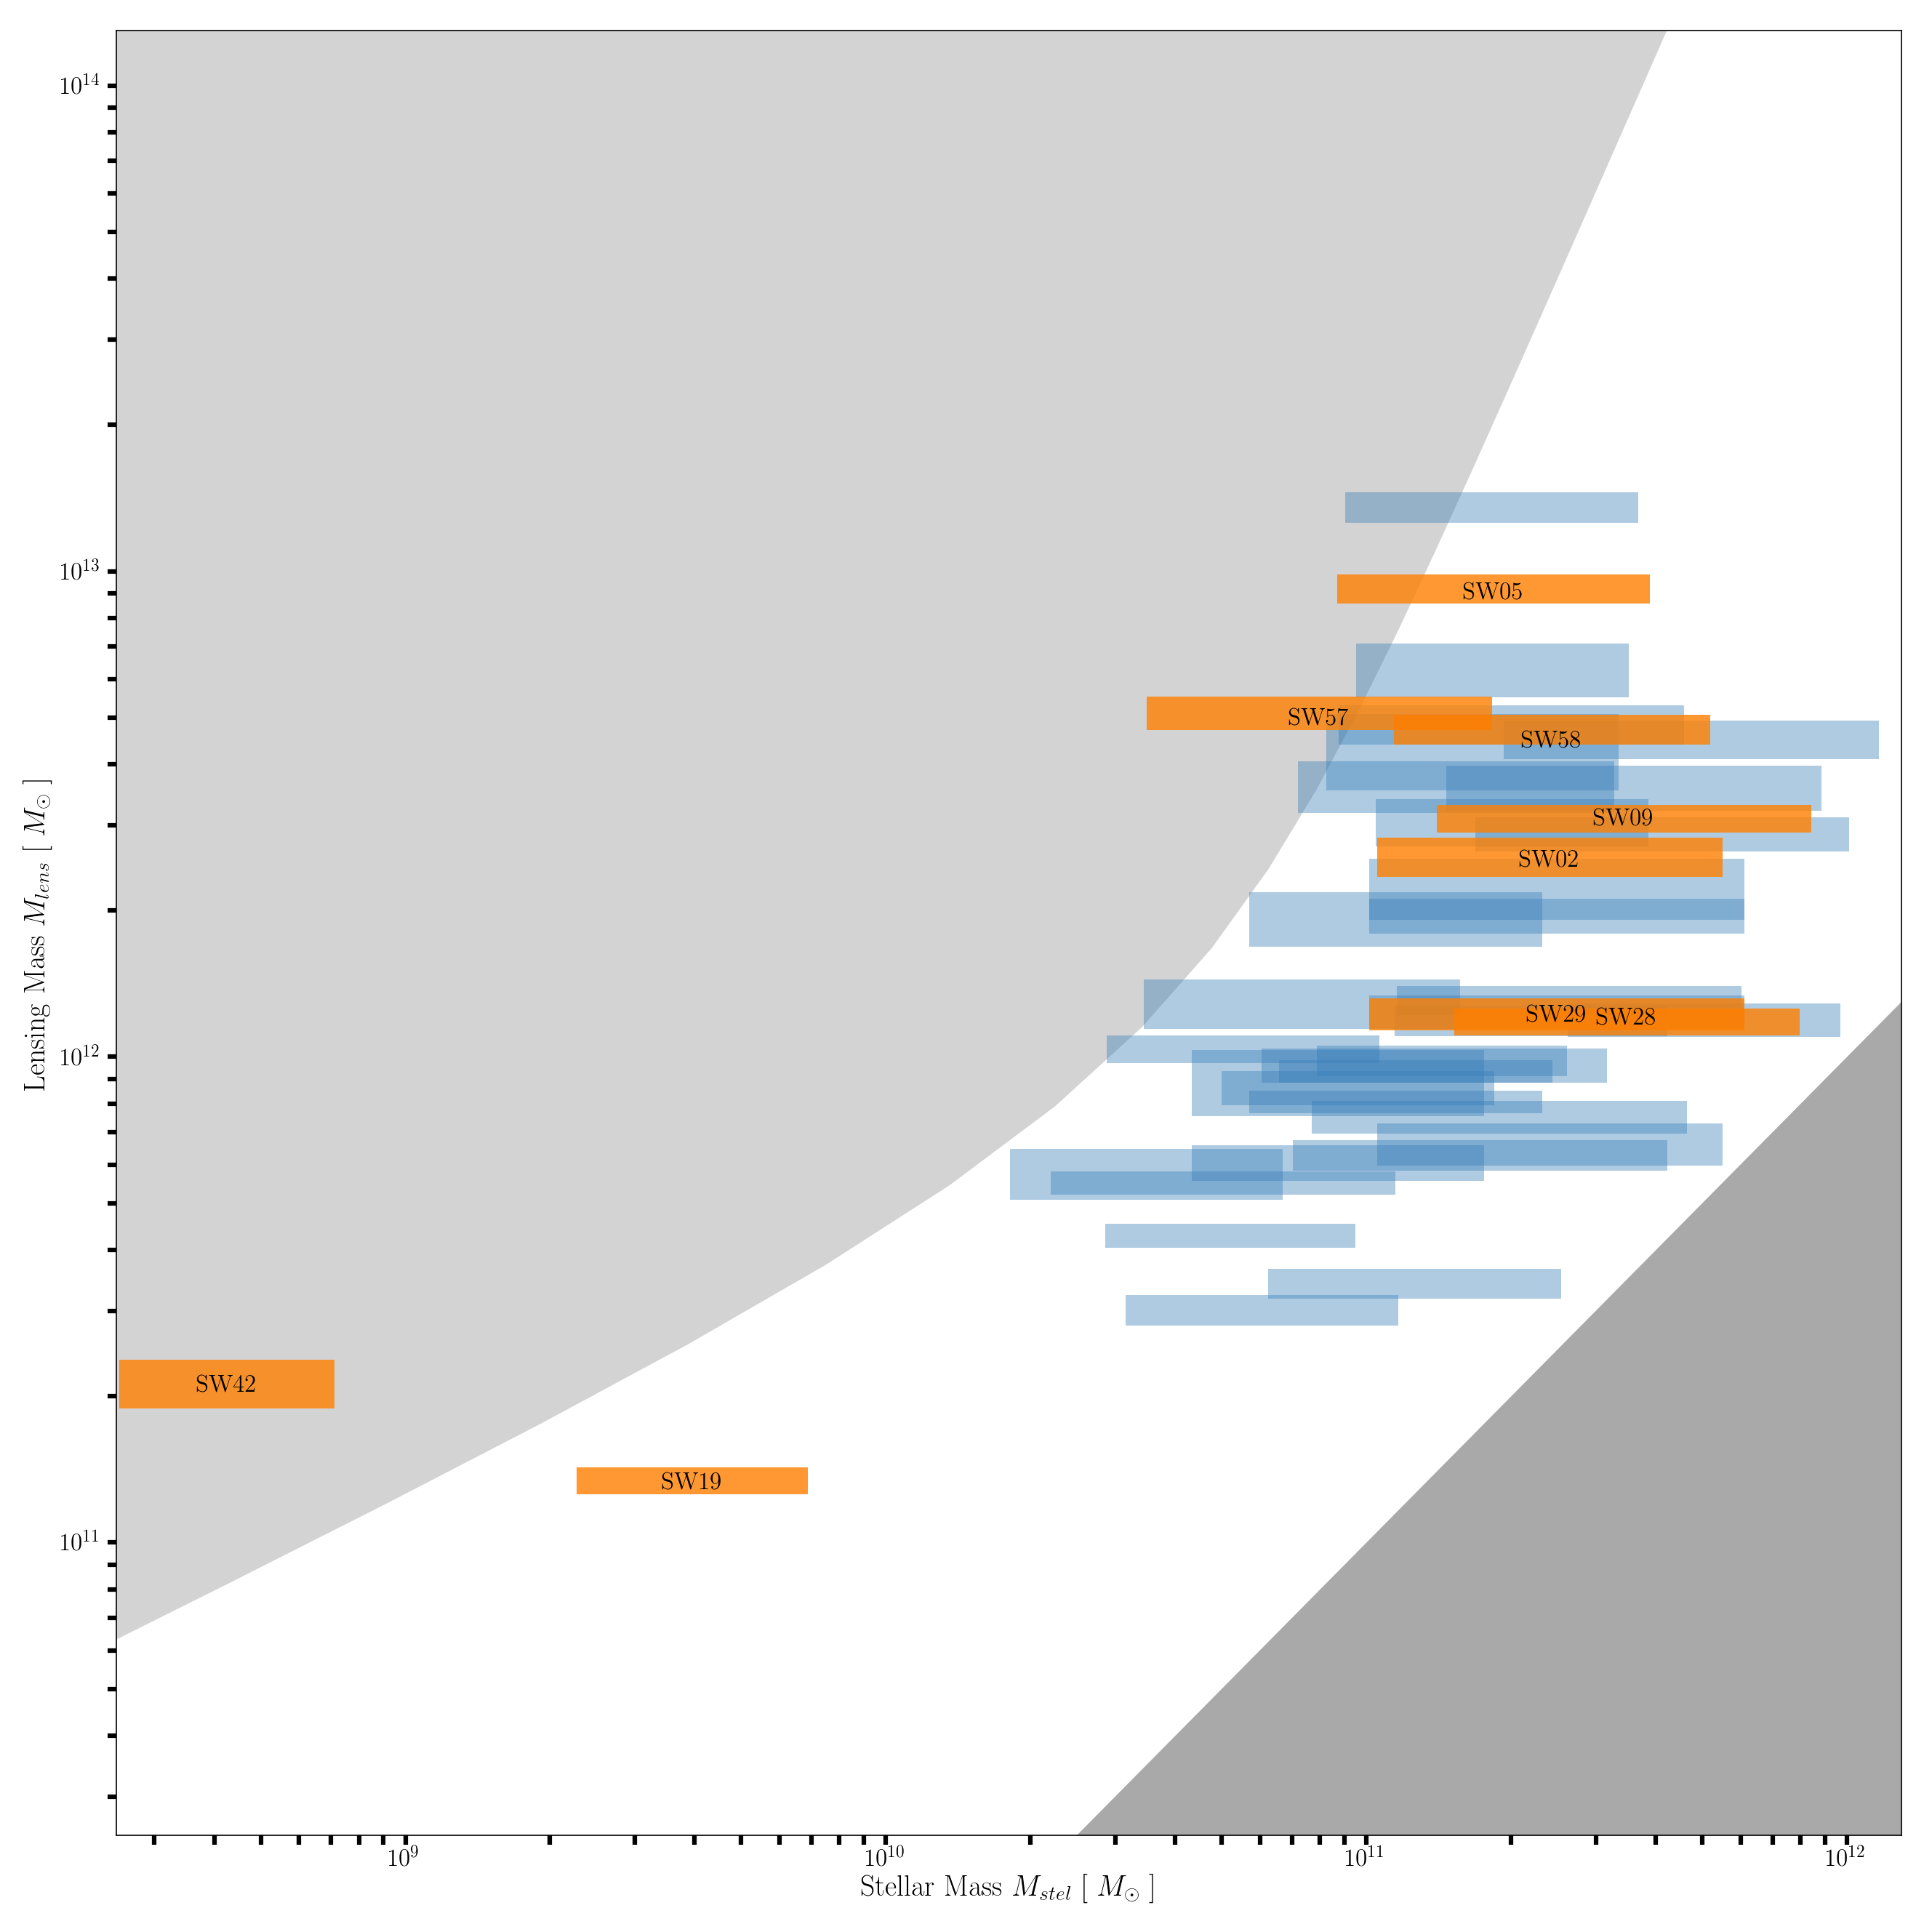
\includegraphics[width=\linewidth]{img/mlens_vs_mstel_one/mstel_vs_mtot_one}
\caption{Total mass in the model against the estimated stellar mass,
  alongside the values for the whole sample.  The lower-right shaded
  region is unphysical according to the stellar-population models,
  because it gives $M<\Mstel$. The upper-left shaded region is
  unphysical according to abundance matching, because it gives
  $M>\Mhalo$.  That is to say, the unshaded region is
  $0<\haloindex<1$. \label{fig:stelmass}}
\end{figure*}

\begin{table*}
  \caption{Categorisation of SW models}
  \label{tab:models}
  
\begin{tabular}{c c c | c c | c c c | c c c}
  \hline
  SWID & ASW id & model id
  
    & \rot{$z_\text{lens}$}

    & \rot{\shortstack[l]{image\\morphology}}
    
    & \multicolumn{1}{|l|}{\rot{\shortstack[l]{unblended\\images}}}
    & \rot{\shortstack[l]{all images\\discernible}}
    & \rot{\shortstack[l]{isolated\\ lens}}
    
    & \rot{\shortstack[l]{synthetic image\\ reasonable}}
    & \rot{\shortstack[l]{mass map\\ reasonable}}
    & \rot{\shortstack[l]{total vs stellar\\ mass ratio}}
  \\ \hline
  SW01 & ASW0004dv8 & J022409.5-105807 & 
    & 
    &  &  & 
    &  &  &  \\
    
  SW02 & ASW000619d & J140522.2+574333 & 0.7
    & LQ
    & \NO & \OK & \NO
    & \OK & \OK & 10 \\
    
  SW03 & ASW0006mea & J142603.2+511421 & 
    & 
    &  &  & 
    &  &  &  \\
    
  SW04 & ASW0009cjs & J142934.2+562541 & 0.5
    & CQ
    & \OK & \NO & \NO
    & \NO & \OK & 74 \\
    
  SW05 & ASW0007k4r & J143454.4+522850 & 0.6
    & IQ
    & \OK & \OK & \OK
    & \OK & \OK & 1.0e+02 \\
    
  SW06 & ASW0008swn & J143627.9+563832 & 0.5
    & LQ
    & \NO & \OK & \OK
    & \OK & \NO & 7 \\
    
  SW07 & ASW0007e08 & J220256.8+023432 & 
    & 
    &  &  & 
    &  &  &  \\
    
  SW08 & ASW00099ed & J020648.0-065639 & 0.8
    & D
    & \OK & \OK & \NO
    & \OK & \OK & 7 \\
    
  SW09 & ASW0002asp & J020832.1-043315 & 1.0
    & SQ
    & \NO & \OK & \OK
    & \OK & \OK & 9 \\
    
  SW10 & ASW0002bmc & J020848.2-042427 & 0.8
    & D
    & \OK & \NO & \OK
    & \NO & \NO & 3 \\
    
  SW11 & ASW0002qtn & J020849.8-050429 & 0.8
    & LQ
    & \NO & \OK & \NO
    & \OK & \OK & 3 \\
    
  SW12 & ASW0003wsu & J022406.1-062846 & 0.4
    & D
    & \OK & \OK & \NO
    & \OK & \OK & 4 \\
    
  SW13 & ASW00047ae & J022805.6-051733 & 0.4
    & LQ
    & \NO & \NO & \NO
    & \NO & \NO & 7 \\
    
  SW14 & ASW0004xjk & J023123.2-082535 & 
    & 
    &  &  & 
    &  &  &  \\
    
  SW15 & ASW0004nan & J084841.0-045237 & 0.3
    & LQ
    & \NO & \OK & \NO
    & \OK & \OK & 8 \\
    
  SW16 & ASW0009bp2 & J140030.2+574437 & 0.4
    & D
    & \NO & \NO & \OK
    & \NO & \OK & 5 \\
    
  SW17 & ASW0005rnb & J140622.9+520942 & 0.7
    & D
    & \OK & \NO & \NO
    & \NO & \OK & 6 \\
    
  SW18 & ASW0007hu2 & J143658.1+533807 & 0.7
    & D
    & \OK & \NO & \OK
    & \NO & \NO & 4 \\
    
  SW19 & ASW0001ld7 & J020642.0-095157 & 0.2
    & IQ
    & \NO & \OK & \NO
    & \NO & \OK & 34 \\
    
  SW20 & ASW0002dx7 & J021221.1-105251 & 0.3
    & IQ
    & \OK & \OK & \OK
    & \NO & \OK & 6 \\
    
  SW21 & ASW0004m3x & J022533.3-053204 & 0.5
    & D
    & \OK & \NO & \NO
    & \NO & \OK & 2 \\
    
  SW22 & ASW0009ab8 & J022716.4-105602 & 0.4
    & D
    &  & \NO & \NO
    & \NO & \OK & 2 \\
    
  SW23 & ASW0003r61 & J023008.6-054038 & 0.6
    & ???
    & ? & ? & ?
    & ? & ? & 23 \\
    
  SW24 & ASW00050sk & J023315.2-042243 & 0.7
    & LQ
    & \NO & \OK & \NO
    & \OK & \OK & 2 \\
    
  SW25 & ASW00007mq & J090308.2-043252 & 
    & 
    &  &  & 
    &  &  &  \\
    
  SW26 & ASW0005ma2 & J135755.8+571722 & 0.8
    & D
    & \OK & \NO & \OK
    & \NO & \NO & 9 \\
    
  SW27 & ASW0006jh5 & J141432.9+534004 & 0.7
    & LQ
    & \NO & \NO & \NO
    & \NO & \OK & 10 \\
    
  SW28 & ASW0007xrs & J143055.9+572431 & 0.7
    & LQ
    & \NO & \OK & \NO
    & \OK & \OK & 3 \\
    
  SW29 & ASW0008qsm & J143838.1+572647 & 0.8
    & SQ
    & \NO & \OK & \OK
    & \OK & \OK & 4 \\
    
  SW30 & ASW0002p8y & J021057.9-084450 & 
    & 
    &  &  & 
    &  &  &  \\
    
  SW31 & ASW00021r0 & J021514.6-092440 & 0.7
    & LQ
    & \NO & \OK & \NO
    & \OK & \OK & 24 \\
    
  SW32 & ASW0004iye & J022359.8-083651 & 
    & 
    &  &  & 
    &  &  &  \\
    
  SW33 & ASW0003s0m & J022745.2-062518 & 0.6
    & D
    & \OK & \OK & \NO
    & \NO & \OK & 17 \\
    
  SW34 & ASW00051ld & J023453.5-093032 & 0.5
    & ???
    & ? & ? & ?
    & ? & ? & 10 \\
    
  SW35 & ASW0004wgd & J084833.2-044051 & 0.8
    & LQ
    & \NO & \OK & \NO
    & \OK & \OK & 5 \\
    
  SW36 & ASW000096t & J090248.4-010232 & 0.4
    & D
    & \OK & \OK & \NO
    & \NO & \OK & 9 \\
    
  SW37 & ASW00086xq & J143100.2+564603 & 
    & 
    &  &  & 
    &  &  &  \\
    
  SW38 & ASW0009cp0 & J143353.6+542310 & 0.8
    & LQ
    & \NO & \OK & \OK
    & \OK & \OK & 9 \\
    
  SW39 & ASW0005qiz & J220215.2+012124 & 
    & 
    &  &  & 
    &  &  &  \\
    
  SW40 & ASW0008wmr & J221306.1+014708 & 
    & 
    &  &  & 
    &  &  &  \\
    
  SW41 & ASW0008xbu & J221519.7+005758 & 0.4
    & IQ
    & \OK & \NO & \OK
    & \OK & \OK & 16 \\
    
  SW42 & ASW00096rm & J221716.5+015826 & 0.1
    & IQ
    & \OK & \OK & \NO
    & \OK & \NO & 5.0e+02 \\
    
  SW43 & ASW0001c3j & J020810.7-040220 & 1.0
    & IQ
    & \NO & \NO & \NO
    & \NO & \OK & 6 \\
    
  SW44 & ASW0002k40 & J021021.5-093415 & 0.4
    & ???
    & ? & ? & ?
    & ? & ? & 34 \\
    
  SW45 & ASW00024id & J021225.2-085211 & 0.8
    & R
    & \NO & \OK & \OK
    & \NO & \OK & 8 \\
    
  SW46 & ASW00024q6 & J021317.6-084819 & 0.5
    & D
    & \OK & \OK & \NO
    & \OK & \OK & 6 \\
    
  SW47 & ASW0003r6c & J022843.0-063316 & 0.5
    & D
    & \OK & \NO & \OK
    & \NO & \OK & 26 \\
    
  SW48 & ASW0000g95 & J090219.0-053923 & 
    & 
    &  &  & 
    &  &  &  \\
    
  SW49 & ASW00007ls & J090319.4-040146 & 
    & 
    &  &  & 
    &  &  &  \\
    
  SW50 & ASW00008a0 & J090333.2-005829 & 
    & 
    &  &  & 
    &  &  &  \\
    
  SW51 & ASW0006e0o & J135724.8+561614 & 
    & 
    &  &  & 
    &  &  &  \\
    
  SW52 & ASW0006a07 & J140027.9+541028 & 
    & 
    &  &  & 
    &  &  &  \\
    
  SW53 & ASW00070vl & J141518.9+513915 & 0.4
    & D
    & \OK & \NO & \OK
    & \NO & \OK & 15 \\
    
  SW54 & ASW0007sez & J142620.8+561356 & 0.5
    & R
    & \NO & \OK & \NO
    & \OK & \OK & 16 \\
    
  SW55 & ASW0007t5y & J142652.8+560001 & 
    & 
    &  &  & 
    &  &  &  \\
    
  SW56 & ASW0007pga & J142843.5+543713 & 0.4
    & D
    & \OK & \NO & \OK
    & \NO & \NO & 18 \\
    
  SW57 & ASW0008pag & J143631.5+571131 & 0.7
    & LQ
    & \NO & \OK & \NO
    & \NO & \NO & 64 \\
    
  SW58 & ASW0007iwp & J143651.6+530705 & 0.6
    & SQ
    & \NO & \NO & \OK
    & \OK & \OK & 19 \\
    
  SW59 & ASW00085cp & J143950.6+544606 & 
    & 
    &  &  & 
    &  &  &  \\
    


  \hline

\end{tabular}

\end{table*}
